\documentclass[11pt,a4paper]{report}

% ---------------------------------------------------------------------------
% Ovaj izvjestaj je namjerno napisan u cistom LaTeX-u (kompajlira se identicno
% na Overleaf-u i lokalno u MiKTeX-u/TeX Live-u) i koristi TikZ za SVE
% dijagrame - nema potrebe za OpenDraw/LibreOffice Draw ili bilo kakvim
% eksternim slikovnim fajlovima. Vidi docs/TODO.txt i PROGRESS_NOTES.txt (u
% korijenu repozitorija) za listu mjesta gdje TREBAS dopuniti stvarne
% rezultate simulacije (oznaceno jasno TODO komentarima ispod).
% ---------------------------------------------------------------------------

\usepackage[utf8]{inputenc}
\usepackage[T1]{fontenc}
\usepackage[croatian]{babel} % najblizi dostupan babel jezik za bosanski (latinica)
\usepackage[margin=2.5cm]{geometry}
\usepackage{graphicx}
\usepackage{amsmath}
\usepackage{amssymb}
\usepackage{booktabs}
\usepackage{array}
\usepackage{xcolor}
\usepackage{listings}
\usepackage{caption}
\usepackage{float}
\usepackage{tikz}
\usetikzlibrary{shapes.geometric,arrows.meta,positioning,fit,backgrounds,calc}
\usepackage[colorlinks=true,linkcolor=blue,citecolor=blue,urlcolor=blue]{hyperref}

\definecolor{codebg}{rgb}{0.96,0.96,0.96}
\definecolor{codecomment}{rgb}{0.4,0.55,0.4}
\definecolor{codekeyword}{rgb}{0.1,0.1,0.7}

\lstdefinestyle{codestyle}{
    backgroundcolor=\color{codebg},
    commentstyle=\color{codecomment},
    keywordstyle=\color{codekeyword}\bfseries,
    basicstyle=\ttfamily\footnotesize,
    breaklines=true,
    showstringspaces=false,
    frame=single,
    numbers=left,
    numberstyle=\tiny,
    xleftmargin=1.5em,
}
\lstset{style=codestyle}

\newcommand{\todobox}[1]{%
  \begin{center}
  \fbox{\begin{minipage}{0.9\textwidth}
  \textbf{TODO (popuniti prije predaje):} #1
  \end{minipage}}
  \end{center}
}

% Privremeni placeholder dok se ne ubace stvarni screenshotovi (svijetla pozadina,
% ne dTwin-ov crni graf) - zamijeniti sa \includegraphics kad slike stignu.
\newcommand{\plotplaceholder}[1]{%
  \begin{tikzpicture}
  \draw[dashed] (0,0) rectangle (12,4);
  \node at (6,2) {\small [graf: \texttt{#1}]};
  \end{tikzpicture}%
}

\begin{document}

\begin{titlepage}
\begin{flushleft}
Univerzitet u Sarajevu\\
Elektrotehnički fakultet\\
\textbf{Strukture i režimi rada elektroenergetskih sistema 2025/2026}
\end{flushleft}

\vspace{6cm}

\begin{center}
{\LARGE \textbf{Dinamički konvertor za Static Var Compensator\\[0.3em] (SVC Type I, SVC Type II)}}\\[0.8em]
{\large natID / dTwin plugin}
\end{center}

\vspace{6cm}

\begin{flushright}
Student:\\
\textbf{Haris Hodžić}\\
Indeks: 19145
\end{flushright}

\vfill

07.07.2026.

\end{titlepage}

\begin{abstract}
Ovaj rad opisuje dizajn i implementaciju dinamičkog konvertora za \emph{Static Var
Compensator} (SVC) uređaje, u obliku plugina (dll) za platformu \textbf{dTwin}, izgrađenog
korištenjem \textbf{natID} okvira (Izudin Dzafic). Konvertor učitava mrežu opisanu u
MATPOWER formatu (\texttt{case9}, \texttt{case30}, \texttt{case118}, \texttt{case300}) i
XML konfiguracijski fajl koji određuje koji čvor (bus) treba biti modeliran kao SVC Type I
(model preko ugla paljenja tiristora), koji kao SVC Type II (model preko susceptanse), a
koji zadržava svoj standardni statički (Slack/PV/PQ) model. Rezultat je diferencijalno-
algebarski (DAE) model u dTwin-ovom \texttt{.dmodl} formatu, spreman za vremensku
simulaciju. Sve matrične operacije koriste natID-ove \texttt{dense} i \texttt{sparse}
matrice; GUI je izgrađen pomoću natGUI biblioteke; konverzija se izvršava u odvojenom
thread-u dok GUI thread u realnom vremenu prikazuje napredak.
\end{abstract}

\tableofcontents

% =============================================================================
\chapter{Uvod}
% =============================================================================

\section{Motivacija}

\emph{Static Var Compensator} (SVC) je uređaj iz porodice FACTS (\emph{Flexible AC
Transmission Systems}) uređaja koji omogućava kontinuiranu regulaciju napona na mjestu
priključenja variranjem svoje efektivne šant (shunt) susceptanse. SVC se sastoji od
tiristorski upravljanog reaktora (TCR - \emph{Thyristor Controlled Reactor}) spojenog
paralelno sa fiksnim kondenzatorom (FC - \emph{Fixed Capacitor})
\cite{acha2004facts,milano2010psms}. Zbog svoje brzine odziva i mogućnosti kontinuirane
regulacije, SVC se široko koristi za podršku naponu, prigušenje oscilacija snage i
povećanje prenosnog kapaciteta mreže.

Cilj ovog projekta je da se, unutar postojećeg dTwin ekosistema za digitalno modeliranje
i simulaciju elektroenergetskih sistema, omogući \textbf{automatska konverzija} statičkog
MATPOWER modela mreže u dinamički DAE model koji na odabranim čvorovima uključuje SVC
Type I i/ili SVC Type II dinamiku, umjesto da se to radi ručno.

\section{Zahtjevi zadatka}

Prema uputstvu predmeta, rješenje mora:
\begin{itemize}
    \item biti napisano u C++ i koristiti \textbf{isključivo} natID-ove \texttt{dense} i
        \texttt{sparse} matrice za sve matrične operacije;
    \item biti isporučeno kao GUI plugin (\texttt{.dll}) za dTwin, korištenjem natGUI
        biblioteke;
    \item omogućiti konfigurisanje preko XML fajla koji određuje koji čvor je kojeg tipa
        (SVC Type I, SVC Type II ili standardni);
    \item raditi konverziju u jednom thread-u, dok se napredak konverzije u realnom
        vremenu prikazuje u GUI-u iz drugog thread-a;
    \item biti testirano na standardnim MATPOWER test slučajevima \texttt{case9},
        \texttt{case30}, \texttt{case118} i \texttt{case300}.
\end{itemize}

\section{Pregled dokumenta}

Poglavlje \ref{ch:teorija} opisuje matematički model SVC Type I i Type II uređaja.
Poglavlje \ref{ch:arhitektura} opisuje arhitekturu implementiranog rješenja. Poglavlje
\ref{ch:implementacija} ulazi u detalje implementacije (parsiranje MATPOWER formata,
izgradnja matrice admitansi, generisanje DAE modela, GUI i threading). Poglavlje
\ref{ch:xml} opisuje format XML konfiguracije. Poglavlje \ref{ch:testiranje} opisuje
testne slučajeve i rezultate. Poglavlje \ref{ch:zakljucak} sadrži zaključak.


% =============================================================================
\chapter{Teorijska pozadina: SVC Type I i Type II}
\label{ch:teorija}
% =============================================================================

\section{Static Var Compensator - princip rada}

SVC uređaj (Slika \ref{fig:svc-shema}) je šant (shunt) uređaj koji se sastoji od
tiristorski upravljanog reaktora (TCR) i fiksnog kondenzatora (FC), povezanih paralelno na
sabirnicu čiji napon treba regulisati. Tiristori u TCR grani se pale sa uglom paljenja
$\sigma$ (mjerenim od prolaska napona kroz nulu), čime se kontroliše koliko dugo struja
teče kroz reaktor u svakoj poluperiodi, a time i efektivna induktivna susceptansa TCR
grane.

\begin{figure}[H]
\centering
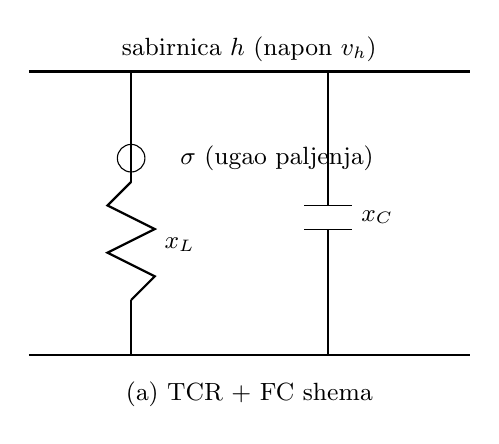
\begin{tikzpicture}[
    every node/.style={font=\small},
    busline/.style={thick},
]
    % bus bar
    \draw[busline] (-0.3,3) -- (5.3,3);
    \node[above] at (2.5,3) {sabirnica $h$ (napon $v_h$)};

    % TCR branch
    \draw[busline] (1,3) -- (1,1.6);
    \draw[busline] (1,1.6) -- (0.7,1.3) -- (1.3,1.0) -- (0.7,0.7) -- (1.3,0.4) -- (1,0.1);
    \node[right] at (1.3,0.8) {$x_L$};
    \draw[busline] (1,0.1) -- (1,-0.6);
    % thyristor symbol (simplified as a switch with angle sigma)
    \node[draw,circle,minimum size=0.35cm,inner sep=0pt] (thy) at (1,1.9) {};
    \node[right] at (1.5,1.9) {$\sigma$ (ugao paljenja)};
    \draw[busline] (-0.3,-0.6) -- (5.3,-0.6);

    % FC branch
    \draw[busline] (3.5,3) -- (3.5,1.3);
    \draw (3.2,1.3) -- (3.8,1.3);
    \draw (3.2,1.0) -- (3.8,1.0);
    \node[right] at (3.8,1.15) {$x_C$};
    \draw[busline] (3.5,1.0) -- (3.5,-0.6);

    \node at (2.5,-1.1) {(a) TCR + FC shema};
\end{tikzpicture}
\hspace{1.5cm}
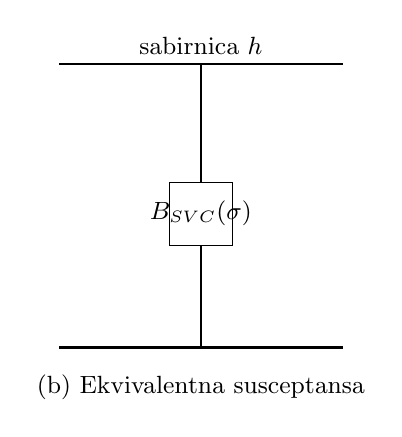
\begin{tikzpicture}[every node/.style={font=\small}]
    \draw[thick] (-0.3,3) -- (3.3,3);
    \node[above] at (1.5,3) {sabirnica $h$};
    \draw[thick] (1.5,3) -- (1.5,1.5);
    \draw (1.1,1.5) rectangle (1.9,0.7);
    \node at (1.5,1.1) {$B_{SVC}(\sigma)$};
    \draw[thick] (1.5,0.7) -- (1.5,-0.6);
    \draw[thick] (-0.3,-0.6) -- (3.3,-0.6);
    \node at (1.5,-1.1) {(b) Ekvivalentna susceptansa};
\end{tikzpicture}
\caption{SVC shema: (a) TCR + FC konfiguracija, (b) ekvivalentni model preko varijabilne
susceptanse $B_{SVC}(\sigma)$. Prilagođeno prema \cite{milano2010psms}, Fig. 19.1.}
\label{fig:svc-shema}
\end{figure}

Efektivna susceptansa SVC-a, kao funkcija ugla paljenja $\sigma$, data je izrazom
(standardna TCR-FC formula, \cite{milano2010psms,acha2004facts}):
\begin{equation}
B_{SVC}(\sigma) = \frac{1}{x_C} - \frac{2\pi - 2\sigma + \sin(2\sigma)}{\pi x_L}
\label{eq:bsvc}
\end{equation}
gdje je $x_L$ induktivna a $x_C$ kapacitivna reaktansa. Za $\sigma = \pi/2$ (TCR potpuno
provodi) dobija se $B_{SVC} = 1/x_C - 1/x_L$, a za $\sigma = \pi$ (TCR potpuno blokiran,
samo kondenzator aktivan) dobija se $B_{SVC} = 1/x_C$ - pozitivna (kapacitivna)
vrijednost, što je i fizički očekivano. Reaktivna snaga koju SVC injektuje u mrežu je:
\begin{equation}
Q_{SVC} = B_{SVC} \cdot v_h^2
\label{eq:qsvc}
\end{equation}

\section{SVC Type I - model preko ugla paljenja}

Kod SVC Type I modela, upravljačka (regulisana) varijabla je direktno ugao paljenja
$\sigma$. Naponski regulator upoređuje mjereni (filtrirani) napon $v_M$ sa referentnim
naponom $v_{ref}$ i preko PI-tipa regulatora (lead-lag) mijenja $\sigma$ (Slika
\ref{fig:svc1-block}).

\begin{figure}[H]
\centering
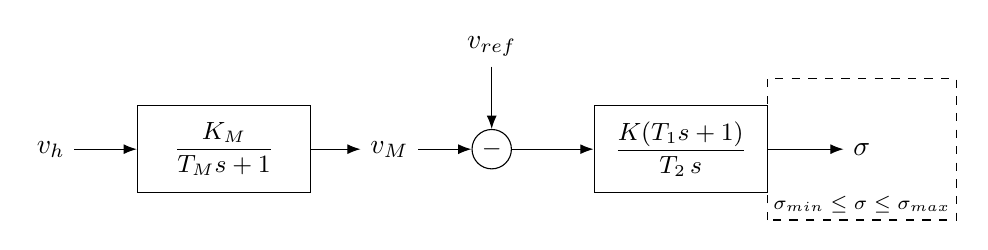
\begin{tikzpicture}[
    block/.style={draw,minimum height=1.1cm,minimum width=2.2cm,align=center,font=\small},
    sum/.style={draw,circle,minimum size=0.5cm,font=\small,inner sep=0pt},
    >=Latex,
]
    \node (vh) at (0,0) {$v_h$};
    \node[block] (meas) at (2.2,0) {$\dfrac{K_M}{T_M s + 1}$};
    \node (vm) at (4.3,0) {$v_M$};
    \node[sum] (s1) at (5.6,0) {$-$};
    \node (vref) at (5.6,1.3) {$v_{ref}$};
    \node[block] (ctrl) at (8.0,0) {$\dfrac{K(T_1 s + 1)}{T_2\, s}$};
    \node (sigma) at (10.3,0) {$\sigma$};

    \draw[->] (vh) -- (meas);
    \draw[->] (meas) -- (vm);
    \draw[->] (vm) -- (s1);
    \draw[->] (vref) -- (s1);
    \draw[->] (s1) -- (ctrl);
    \draw[->] (ctrl) -- (sigma);
    \draw[dashed] (9.1,-0.9) rectangle (11.5,0.9);
    \node[font=\scriptsize] at (10.3,-0.7) {$\sigma_{min} \le \sigma \le \sigma_{max}$};
\end{tikzpicture}
\caption{SVC Type I - blok dijagram regulatora (prilagođeno prema \cite{milano2010psms}, Fig. 19.2).}
\label{fig:svc1-block}
\end{figure}

Sistem diferencijalno-algebarskih jednačina (Milano, jed. 19.3 \cite{milano2010psms}):
\begin{align}
\dot{v}_M &= \frac{K_M v_h - v_M}{T_M} \label{eq:svc1-vm}\\
\dot{\sigma} &= -K_D + \frac{K T_1}{T_2 T_M}\left(v_M - K_M v_h\right) + \frac{K}{T_2}\left(v_{ref} - v_M\right) \label{eq:svc1-sigma}\\
Q_h &= B_{SVC}(\sigma)\, v_h^2 \label{eq:svc1-q}
\end{align}
Stanje $\sigma$ ima anti-windup limiter (Tabela \ref{tab:svc1-params}): kada $\sigma$
dostigne $\sigma_{min}$ ili $\sigma_{max}$, njegov izvod se privremeno zaključava na nulu
(implementirano preko logičke zastavice, vidi Poglavlje \ref{ch:implementacija}).

\begin{table}[H]
\centering
\caption{Parametri SVC Type I (default vrijednosti, Milano Table D.10 \cite{milano2010psms})}
\label{tab:svc1-params}
\begin{tabular}{@{}llc@{}}
\toprule
Varijabla & Opis & Default vrijednost \\
\midrule
$K$ & Pojačanje regulatora & $10.0$ rad/pu \\
$K_D$ & Integralno odstupanje & $0.0$ \\
$K_M$ & Pojačanje mjerenja & $1.0$ pu/pu \\
$T_1$ & Vremenska konstanta (tranzijentna) & $0.05$ s \\
$T_2$ & Vremenska konstanta regulatora & $0.01$ s \\
$T_M$ & Vremensko kašnjenje mjerenja & $0.01$ s \\
$x_L$ & Induktivna reaktansa & $0.1$ pu \\
$x_C$ & Kapacitivna reaktansa & $0.1$ pu \\
$\sigma_{max}$ & Maksimalni ugao paljenja & $\pi$ rad \\
$\sigma_{min}$ & Minimalni ugao paljenja & $-\pi$ rad \\
\bottomrule
\end{tabular}
\end{table}

\section{SVC Type II - model preko susceptanse}

SVC Type II model pojednostavljuje regulaciju pretpostavljajući da je upravljačka
varijabla direktno efektivna susceptansa $B_{SVC}$, a ne ugao paljenja (Slika
\ref{fig:svc2-block}).

\begin{figure}[H]
\centering
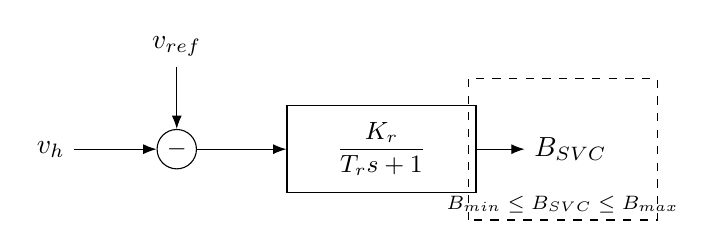
\begin{tikzpicture}[
    block/.style={draw,minimum height=1.1cm,minimum width=2.4cm,align=center,font=\small},
    sum/.style={draw,circle,minimum size=0.5cm,font=\small,inner sep=0pt},
    >=Latex,
]
    \node (vh) at (0,0) {$v_h$};
    \node[sum] (s1) at (1.6,0) {$-$};
    \node (vref) at (1.6,1.3) {$v_{ref}$};
    \node[block] (ctrl) at (4.2,0) {$\dfrac{K_r}{T_r s + 1}$};
    \node (b) at (6.6,0) {$B_{SVC}$};

    \draw[->] (vh) -- (s1);
    \draw[->] (vref) -- (s1);
    \draw[->] (s1) -- (ctrl);
    \draw[->] (ctrl) -- (b);
    \draw[dashed] (5.3,-0.9) rectangle (7.7,0.9);
    \node[font=\scriptsize] at (6.5,-0.7) {$B_{min} \le B_{SVC} \le B_{max}$};
\end{tikzpicture}
\caption{SVC Type II - blok dijagram regulatora (prilagođeno prema \cite{milano2010psms}, Fig. 19.3).}
\label{fig:svc2-block}
\end{figure}

Diferencijalna jednačina (Milano, jed. 19.4 \cite{milano2010psms}):
\begin{align}
\dot{B}_{SVC} &= \frac{K_r (v_{ref} - v_h) - B_{SVC}}{T_r} \label{eq:svc2-b}\\
Q_h &= B_{SVC}\, v_h^2 \label{eq:svc2-q}
\end{align}
Susceptansa $B_{SVC}$ takođe ima anti-windup limiter između $B_{min}$ i $B_{max}$.

\begin{table}[H]
\centering
\caption{Parametri SVC Type II (default vrijednosti, Milano Table D.11 \cite{milano2010psms})}
\label{tab:svc2-params}
\begin{tabular}{@{}llc@{}}
\toprule
Varijabla & Opis & Default vrijednost \\
\midrule
$K_r$ & Pojačanje regulatora & $10.0$ pu/pu \\
$T_r$ & Vremenska konstanta regulatora & $0.05$ s \\
$B_{max}$ & Maksimalna susceptansa & $0.20$ pu \\
$B_{min}$ & Minimalna susceptansa & $-0.05$ pu \\
\bottomrule
\end{tabular}
\end{table}

Prema Milanu \cite{milano2010psms}, Type II model pokazuje nultu statičku grešku (zbog
integralnog djelovanja) ali sa izraženijim visokofrekventnim oscilacijama u odnosu na Type
I model - ovo je i eksperimentalno provjereno u sklopu izrade ovog projekta (vidi
Poglavlje \ref{ch:testiranje}).

\section{Inicijalizacija SVC-a}

Kako Milano navodi \cite{milano2010psms}, SVC uređaji se tipično inicijalizuju
\emph{nakon} rješavanja tokova snage: referentni napon $v_{ref}$ se postavlja na
vrijednost napona koju je tokovi snage već izračunao (ili na napon generatora, ako čvor
prije konverzije ima priključen generator). U implementiranom rješenju, ako XML
konfiguracija ne navodi eksplicitnu vrijednost \texttt{vref}, ona se automatski uzima iz
MATPOWER \texttt{.m} fajla (napon generatora $V_g$ ako postoji na tom čvoru, inače napon
sabirnice $V_m$) - vidi Poglavlje \ref{ch:implementacija}.


% =============================================================================
\chapter{Arhitektura rješenja}
\label{ch:arhitektura}
% =============================================================================

\section{Pregled}

Rješenje je organizovano kao dvije natID/CMake "solution" cjeline (Slika
\ref{fig:arhitektura}):
\begin{itemize}
    \item \textbf{SVCPluginSol} - sam dTwin plugin (\texttt{svcConv.dll}), koji
        implementira \texttt{sc::IPlugin} interfejs i sadrži cjelokupnu logiku konverzije;
    \item \textbf{TestSVCPluginSol} - samostalna host aplikacija za testiranje plugina
        izvan pune dTwin aplikacije (isti obrazac kao natID-ov \texttt{TestEQPlugin}
        primjer).
\end{itemize}

\begin{figure}[H]
\centering
\resizebox{\textwidth}{!}{%
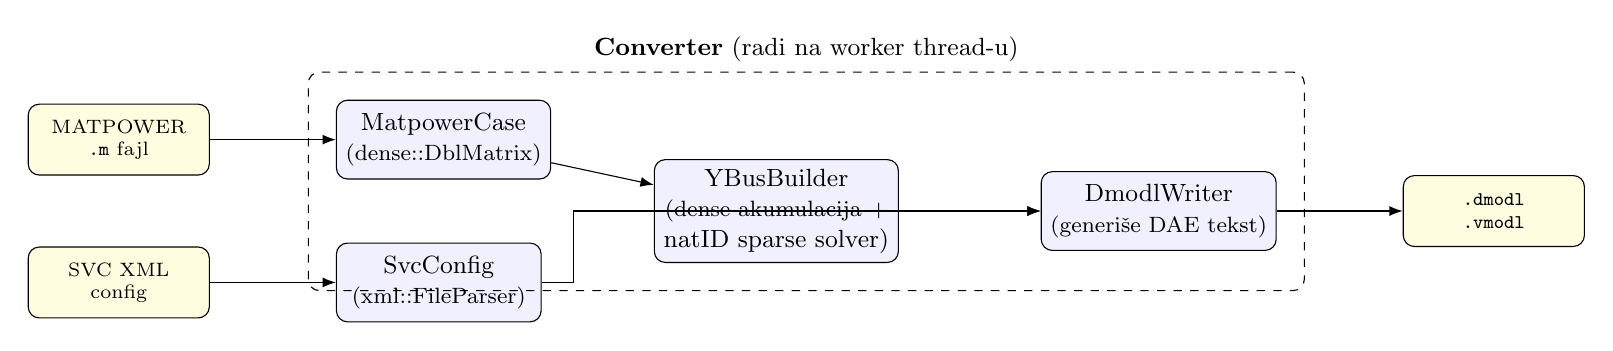
\begin{tikzpicture}[
    block/.style={draw,rounded corners,minimum height=1cm,minimum width=2.6cm,align=center,font=\small,fill=blue!6},
    io/.style={draw,rounded corners,minimum height=0.9cm,minimum width=2.3cm,align=center,font=\scriptsize,fill=yellow!12},
    >=Latex,
    node distance=0.9cm and 1.0cm,
]
    \node[io] (mfile) {MATPOWER\\\texttt{.m} fajl};
    \node[io,below=of mfile] (xmlfile) {SVC XML\\config};

    \node[block,right=1.6cm of mfile] (mpcase) {MatpowerCase\\\footnotesize(dense::DblMatrix)};
    \node[block,right=1.6cm of xmlfile] (svccfg) {SvcConfig\\\footnotesize(xml::FileParser)};

    \node[block, right=2.7cm of $(mpcase)!0.5!(svccfg)$] (ybus) {YBusBuilder\\\footnotesize(dense akumulacija +\\natID sparse solver)};

    \node[block, right=1.8cm of ybus] (dmodl) {DmodlWriter\\\footnotesize(generiše DAE tekst)};

    \node[io, right=1.6cm of dmodl] (out) {\texttt{.dmodl}\\\texttt{.vmodl}};

    \draw[->] (mfile) -- (mpcase);
    \draw[->] (xmlfile) -- (svccfg);
    \draw[->] (mpcase) -- (ybus);
    \draw[->] (svccfg.east) -- ++(0.4,0) |- (dmodl.west);
    \draw[->] (ybus) -- (dmodl);
    \draw[->] (dmodl) -- (out);

    \node[draw,dashed,rounded corners,fit=(mpcase)(ybus)(dmodl),inner sep=0.35cm,label={[font=\small]above:\textbf{Converter} (radi na worker thread-u)}] (convbox) {};
\end{tikzpicture}%
}
\caption{Arhitektura toka podataka konvertora.}
\label{fig:arhitektura}
\end{figure}

\section{GUI i threading arhitektura}

Plugin GUI je izgrađen po obrascu natID-ovog \texttt{EQPlugin} primjera: prozor
(\texttt{WindowPlugin}) sadrži tabovanu vrpcu (\texttt{TabView}) sa dva view-a:
\texttt{ViewConv} (izbor ulaznog \texttt{.m} fajla, XML konfiguracije i izlaznog
\texttt{.dmodl} fajla, dugme \emph{Convert}, indikator napretka) i \texttt{ViewOptions}
(opcionalno prepisivanje Header/solver opcija).

Konverzija (koja za \texttt{case300} može trajati primjetno vrijeme zbog generisanja
NLE jednačina za 300 čvorova) izvršava se na zasebnom \texttt{std::thread}-u, kako GUI ne
bi "zamrznuo" tokom konverzije (Slika \ref{fig:threading}). Napredak se iz worker thread-a
šalje nazad na glavni (GUI) thread isključivo preko
\texttt{gui::thread::asyncExecInMainThread} mehanizma natID-a - direktan pristup GUI
elementima sa worker thread-a nikad se ne dešava, čime se izbjegavaju tipični
"race condition" problemi.

\begin{figure}[H]
\centering
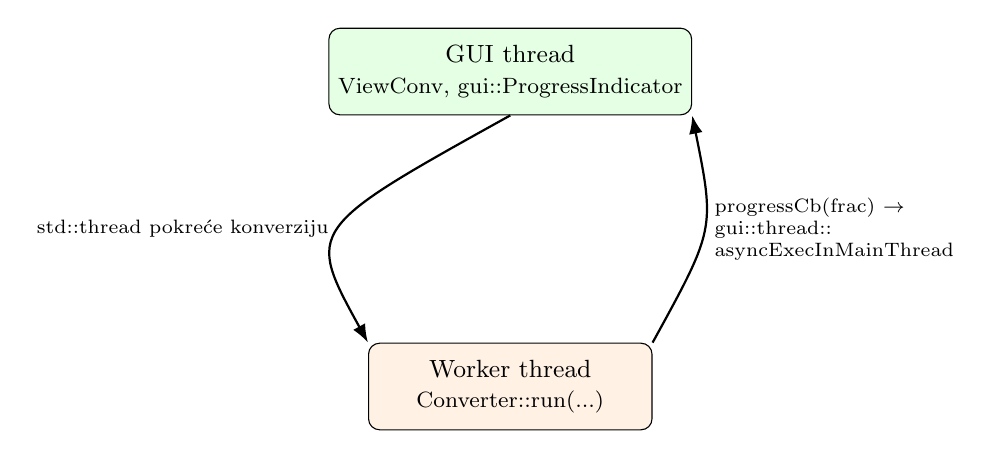
\begin{tikzpicture}[
    block/.style={draw,rounded corners,minimum height=1.1cm,minimum width=3.6cm,align=center,font=\small},
    >=Latex,
]
    \node[block,fill=green!10] (gui) at (0,2) {GUI thread\\\footnotesize ViewConv, gui::ProgressIndicator};
    \node[block,fill=orange!10] (worker) at (0,-2) {Worker thread\\\footnotesize Converter::run(...)};

    \draw[->,thick] (gui.south) .. controls (-2.6,0) and (-2.6,0) .. (worker.north west)
        node[midway,left,font=\scriptsize] {std::thread pokreće konverziju};

    \draw[->,thick] (worker.north east) .. controls (2.6,0) and (2.6,0) .. (gui.south east)
        node[midway,right,font=\scriptsize,align=left] {progressCb(frac) $\rightarrow$\\gui::thread::\\asyncExecInMainThread};
\end{tikzpicture}
\caption{Threading model: konverzija i GUI ažuriranje.}
\label{fig:threading}
\end{figure}

\section{Zašto puni C++ pipeline (bez Python predobrade)}

Prošlogodišnji seminarski radovi na sličnu temu (statički konvertor tokova snage) su
matematičku konverziju MATPOWER $\to$ \texttt{.dmodl} radili u Python skripti, koja bi se
pokretala odvojeno od natID GUI plugina. U ovom projektu je taj pristup namjerno
\textbf{izbjegnut}: cjelokupan pipeline (parsiranje \texttt{.m} fajla, izgradnja matrice
admitansi, generisanje DAE teksta) implementiran je unutar C++ plugina, koristeći
isključivo natID-ove \texttt{dense} i \texttt{sparse} matrice, u skladu sa eksplicitnim
zahtjevom uputstva predmeta.


% =============================================================================
\chapter{Implementacija}
\label{ch:implementacija}
% =============================================================================

\section{Parsiranje MATPOWER formata (\texttt{MatpowerCase})}

Klasa \texttt{MatpowerCase} čita \texttt{mpc.baseMVA}, \texttt{mpc.bus},
\texttt{mpc.gen} i \texttt{mpc.branch} blokove iz \texttt{.m} fajla (linija-po-linija
parser, tolerantan na MATLAB-stil komentare \texttt{\%}), i smješta ih u tri
\texttt{dense::DblMatrix} objekta (retci = čvorovi/generatori/grane, kolone prema
standardnom MATPOWER \texttt{caseformat}-u).

\section{Izgradnja matrice admitansi (\texttt{YBusBuilder})}

Matrica admitansi $Y_{bus} = G + jB$ gradi se iz podataka o granama (otpor, reaktansa,
susceptansa, prenosni odnos i fazni pomak transformatora) standardnom formulom za
$\pi$-model dalekovoda/transformatora. Zbog toga što natID-ov \texttt{sparse::IDblMatrix}
interfejs ne nudi mogućnost čitanja proizvoljnog elementa nazad nakon sastavljanja (samo
\texttt{addTriple} + rješavanje sistema + čitanje rješenja preko \texttt{x(i)}), akumulacija
$G$/$B$ vrijednosti radi se u \texttt{dense::DblMatrix} scratch matricama (dimenzije
$N\times N$, gdje je i najveći test slučaj, \texttt{case300}, i dalje trivijalno mali za
gustu reprezentaciju).

natID-ov \textbf{sparse} solver (\texttt{sparse::createDblSolver}, \texttt{addTriple},
\texttt{factorize}, \texttt{solve}, \texttt{x(i)}) se ipak koristi na netrivijalan način:
za jednokratno rješavanje linearizovanog DC tokova snage sistema $B' \theta = P$ (gdje je
red/kolona slack čvora zamijenjena jediničnim retkom), radi dobijanja realističnije
početne procjene uglova napona (umjesto "flat start"-a za sve čvorove) u generisanom
\texttt{Vars} bloku. Ako rješavanje ne uspije, tiho se vraća na flat start - ovo nikad ne
utiče na tačnost samog DAE modela, samo na kvalitet početnog nagađanja.

\section{Generisanje DAE modela (\texttt{DmodlWriter})}

Za svaki čvor mreže generiše se:
\begin{itemize}
    \item ako čvor \textbf{nije} naveden u SVC XML konfiguraciji: standardni statički
        model (Slack: fiksni $v,\varphi$; PV: bezuslovna regulacija napona na zadatu
        vrijednost - bez provjere granice reaktivne snage generatora, radi jednostavnosti;
        PQ: fiksna $P,Q$ injekcija);
    \item ako \textbf{jeste} naveden: SVC Type I ili Type II dinamički model (jednačine
        \ref{eq:svc1-vm}-\ref{eq:svc1-q} ili \ref{eq:svc2-b}-\ref{eq:svc2-q}), gdje
        algebarska jednačina reaktivne snage zamjenjuje standardnu jednačinu bilansa
        reaktivne snage na tom čvoru.
\end{itemize}

Generisani model koristi \texttt{Model[type=DAE]} sekciju sa \texttt{Vars}, \texttt{Params},
\texttt{ODEs} (samo za SVC čvorove) i \texttt{NLEs} (za sve čvorove). Naponi se
predstavljaju u \textbf{polarnim koordinatama} ($v_i$, $\varphi_i$), a $Y_{bus}$ matrica se
u fajl upisuje u polarnom obliku ($|Y_{ik}|$, $\angle Y_{ik}$) - ovo je promjena u odnosu
na raniju verziju generatora koja je koristila pravougaone koordinate ($e_i,f_i$) i
zasebnu \texttt{PostProc} sekciju; razlog promjene je opisan u odjeljku
\ref{sec:postproc-bug}.

Primjer generisanih parametara i jednačina za jedan SVC Type II čvor (bus 9,
\texttt{case9}) - ovo je \textbf{stvaran isječak}, dobijen kompajliranjem projekta (MSVC,
Visual Studio Build Tools 2022) i pokretanjem konverzije na \texttt{case9.m} +
\texttt{svc\_config\_case9.xml}, ne ručno napisan primjer:
\begin{lstlisting}[language=bash,caption={Stvaran isječak generisanog \texttt{.dmodl} sadržaja za SVC Type II čvor (bus 9)},label={lst:dmodl-svc2}]
// Node 9 - SVC Type II
P_9_load = 1.25000000; Q_9_load = 0.50000000;
P_9_inj_spec = -1.25000000;
vref_9 = 1.00000000 [out=true];
Kr_9 = 10.00000000; Tr_9 = 0.05000000;
bMax_9 = 0.20000000; bMin_9 = -0.05000000;
...
ODEs:
	bSvc_9' = (Kr_9*(vref_9 - v_9) - bSvc_9)/Tr_9
...
NLEs:
	v_9*v_4*absY_9_4*cos(phi_9-phi_4-angleY_9_4) + ... - P_9_inj_spec = 0
	v_9*v_4*absY_9_4*sin(phi_9-phi_4-angleY_9_4) + ...
		- bSvc_9*(v_9*v_9) + Q_9_load = 0
	vh_9 - v_9 = 0
	q_9 - bSvc_9*(v_9*v_9) = 0
\end{lstlisting}

Posljednja dva reda (\texttt{vh\_9}, \texttt{q\_9}) su izvedene veličine (napon i
injektirana reaktivna snaga, korištene za grafike u \texttt{.vmodl} fajlu) definisane kao
obične algebarske promjenljive sa pratećom NLE jednačinom, umjesto preko \texttt{PostProc}
sekcije - vidi odjeljak \ref{sec:postproc-bug} za razlog ove odluke.

Vrijednosti $Y_{bus}$ matrice u generisanom fajlu (npr. $B_{1,1}=-17.3611$, $B_{4,4}=-39.3089$,
$B_{9,9}=-17.3382$, prije konverzije u polarni oblik) su provjerene i \textbf{poklapaju se
tačno} sa vrijednostima iz prošlogodišnjeg (Python) konvertora za isti \texttt{case9}
slučaj, što potvrđuje ispravnost implementacije izgradnje matrice admitansi. Kompletan
generisani fajl (\texttt{case9\_svc.dmodl}, 6749 bajtova) i pripadajući
\texttt{case9\_svc.vmodl} nalaze se u \texttt{src/TestSVCPlugin/res/testData/output/} u
repozitoriju, zajedno sa istim izlazima za \texttt{case30}, \texttt{case118} i
\texttt{case300}.

\section{XML parsiranje}

XML konfiguracija se parsira preko natID-ovog \texttt{xml::FileParser} (DOM stil
parsiranja, \texttt{getRootNode()}\allowbreak/\allowbreak\texttt{getChildNode()}\allowbreak/\allowbreak\texttt{getAttribValue()}),
isti obrazac kao u natID primjeru \texttt{04\_XmlIntro}.

\section{Build sistem (CMake)}

Oba rješenja (\texttt{SVCPluginSol}, \texttt{TestSVCPluginSol}) koriste identičnu CMake
strukturu kao natID-ovi primjeri (\texttt{EQPlugin}/\texttt{TestEQPlugin}): jedan
"solution" \texttt{CMakeLists.txt} koji uključuje zajedničke natID komponente
(\texttt{Common.cmake}, \texttt{natGUI.cmake}, \texttt{MatrixLib.cmake}, ...) i po jedan
projekt-specifični \texttt{*.cmake} fajl.

Tokom analize primijećeno je da referentni \texttt{EQPlugin.cmake} na kraju poziva
funkciju \texttt{setIDEPropertiesFor\allowbreak Lib(...)} koja \textbf{ne postoji} ni u
jednoj \texttt{*.cmake} datoteci unutar \texttt{natID.SDK/DevEnv} (postoje samo
\texttt{setIDEPropertiesFor\allowbreak Executable} i
\texttt{setIDEPropertiesFor\allowbreak GUIExecutable}) - ovaj
poziv bi prouzrokovao grešku "Unknown CMake command" pri konfigurisanju. U vlastitom
\texttt{SVCPlugin.cmake} taj poziv je izostavljen (uz komentar objašnjenja).

\section{Napomena o instaliranom natID.SDK-u (za reprodukciju build-a)}
\label{sec:sdk-napomena}

Prilikom prve stvarne kompilacije (MSVC, Visual Studio Build Tools 2022) otkriveno je da
instalirana kopija \texttt{natID.SDK}-a ne sadrži dva zaglavlja koja \texttt{sc/IPlugin.h}
(i primjeri iz \texttt{natID.Examples}) očekuju: \texttt{arch/MemoryOut.h} i
\texttt{syst/LibraryLoader.h} (ovo bi spriječilo kompajliranje \emph{bilo kojeg} natID
dTwin plugina na ovoj instalaciji, uključujući i sam \texttt{EQPlugin} primjer, ne samo
ovaj projekat). Za ovaj projekat su dodana dva minimalna, samostalna zaglavlja
(\texttt{MemoryOut} kao jednostavan rastući memorijski bafer; \texttt{LibraryLoader} kao
tanak omotač oko \texttt{LoadLibrary}/\texttt{GetProcAddress}) direktno u
\texttt{natID.SDK/Common/Include} instalacije korištene za build (nisu dio ovog
repozitorija - ne mijenjaju se postojeći SDK fajlovi, samo se dodaju dva nedostajuća).
\textbf{Ako se projekat kompajlira na drugom sistemu (npr. macOS) sa kompletnom/drugom
verzijom natID.SDK-a}, prvo provjeriti da li ta zaglavlja već postoje - ako postoje,
reconstruisane verzije nije potrebno dodavati.

% =============================================================================
\chapter{XML konfiguracijski format}
\label{ch:xml}
% =============================================================================

Format XML konfiguracije (\texttt{svc\_config\_case*.xml}) omogućava potpunu kontrolu nad
tim koji čvor je kojeg tipa, kao i nad parametrima regulatora i opcijama simulacije:

\begin{lstlisting}[language=XML,caption={Struktura SVC XML konfiguracije (primjer za \texttt{case9})},label={lst:xml-config}]
<SVCConverterConfig>
  <Files>
    <InputFile path="case9.m"/>
    <OutputFile name="case9_svc" directory="./output/"/>
  </Files>
  <Simulation>
    <maxIter>100</maxIter> <report>AllDetails</report>
    <startTime>0</startTime> <dTime>0.01</dTime> <endTime>10</endTime>
    <method>RK2</method>
  </Simulation>
  <Options>
    <EnableNLEComments>true</EnableNLEComments>
    <GeneratorLimits>true</GeneratorLimits>
    <UseDCAngleInit>true</UseDCAngleInit>
  </Options>
  <DefaultsSVCTypeI K="10.0" KD="0.0" KM="1.0" T1="0.05" T2="0.01"
                    TM="0.01" xL="0.1" xC="0.1"
                    sigmaMax="3.14159" sigmaMin="-3.14159"/>
  <DefaultsSVCTypeII Kr="10.0" Tr="0.05" bMax="0.20" bMin="-0.05"/>
  <SVCNodes>
    <Node bus="5" type="SVCTypeI"  vref="1.02"/>
    <Node bus="9" type="SVCTypeII" vref="1.00"/>
  </SVCNodes>
</SVCConverterConfig>
\end{lstlisting}

Svaki bus koji NIJE naveden pod \texttt{<SVCNodes>} zadržava svoj originalni statički
model iz \texttt{.m} fajla. Svaki atribut na elementu \texttt{<Node>} koji nije eksplicitno
naveden preuzima vrijednost iz odgovarajućeg \texttt{<DefaultsSVCTypeI>} /
\texttt{<DefaultsSVCTypeII>} elementa (Milano Table D.10/D.11).


% =============================================================================
\chapter{Testiranje}
\label{ch:testiranje}
% =============================================================================

\section{Test slučajevi}

Konvertor je pripremljen za četiri standardna MATPOWER test slučaja. Tabela
\ref{tab:test-cases} prikazuje odabrane SVC čvorove za svaki slučaj (svi su birani među
originalno PQ/opterećenim čvorovima, isti princip kao u Milanovom IEEE14 primjeru gdje je
SVC postavljen na bus 9).

\begin{table}[H]
\centering
\caption{Test slučajevi i pozicije SVC čvorova}
\label{tab:test-cases}
\begin{tabular}{@{}lcc@{}}
\toprule
Test slučaj & SVC Type I (bus) & SVC Type II (bus) \\
\midrule
case9   & 5  & 9  \\
case30  & 7  & 8  \\
case118 & 11 & 16 \\
case300 & 9  & 13 \\
\bottomrule
\end{tabular}
\end{table}

\section{Validacija jednačina prije implementacije}

Prije ugradnje SVC jednačina u C++ generator, matematički model je nezavisno validiran
pomoću kratke Python skripte (van repozitorija projekta - koristi se isključivo kao
pomoćni alat, ne kao dio rješenja). Skripta provjerava:
\begin{enumerate}
    \item da $B_{SVC}(\sigma)$ (jed. \ref{eq:bsvc}) daje ispravne vrijednosti na fizičkim
        granicama ($\sigma=\pi/2$ i $\sigma=\pi$);
    \item da oba regulatora (Type I i Type II) reaguju u ispravnom smjeru (više
        kapacitivne podrške) nakon pada napona.
\end{enumerate}

Granice $\sigma_{max}/\sigma_{min}$ i $B_{max}/B_{min}$ (Milano Table D.10/D.11) se
generišu kao \texttt{Params} u izlaznom \texttt{.dmodl} fajlu radi potpunosti podataka, ali
se ne provode kao aktivno ograničenje (anti-windup) unutar same DAE simulacije - ranija
verzija generatora je imala \texttt{Limits:} sekciju sa if/else prebacivanjem stanja na
granicu, ali je uklonjena tokom istrage pada aplikacije opisane u odjeljku
\ref{sec:postproc-bug} (naknadno je utvrđeno da to nije bio stvarni uzrok pada, ali
pojednostavljenje je zadržano jer nije bilo neophodno za osnovnu funkcionalnost).

Ova provjera je otkrila i ispravila stvarnu grešku znaka u prvobitnoj rekonstrukciji
jednačine \ref{eq:bsvc} (OCR ekstrakcija teksta iz PDF knjige je izgubila $\pi$ simbole u
originalnoj formuli) - detaljno objašnjeno u \texttt{PROGRESS\_NOTES.txt} u korijenu
repozitorija.

\section{Rezultati simulacije}

\subsection{Verifikacija pipeline-a (konverzija)}

Cijeli konverzijski pipeline je uspješno kompajliran (MSVC 19.44 / Visual Studio Build
Tools 2022, natID SDK) i pokrenut end-to-end za sva četiri test slučaja (\texttt{case9},
\texttt{case30}, \texttt{case118}, \texttt{case300}), i preko samostalnog konzolnog test
harness-a (direktan poziv \texttt{Converter::run(...)}, van GUI-a) i preko pravog
\texttt{svcConv.dll} plugina učitanog unutar dTwin aplikacije. Vrijednosti $Y_{bus}$
matrice za \texttt{case9} tačno se poklapaju sa prošlogodišnjim (nezavisno implementiranim)
konvertorom za isti test slučaj (vidi Poglavlje \ref{ch:implementacija}, Listing
\ref{lst:dmodl-svc2}).

\paragraph{Otklonjen pad aplikacije pri otvaranju generisanog modela.}
\label{sec:postproc-bug}
Tokom testiranja u
pravom dTwin okruženju otkriven je pad aplikacije (crash, kod izuzetka
\texttt{0xc0000409}) koji se dešavao isključivo pri otvaranju generisanih \texttt{.dmodl}
fajlova većih razmjera (\texttt{case9} i veći), a ne i kod manjih referentnih modela
(npr. SDK-ov vlastiti \texttt{PendulumDAE.dmodl}). Sistematskom izolacijom (preko
tridesetak ciljanih test fajlova, upoređivanjem sa vlastitim primjerima iz natID SDK-a i
prošlogodišnjim konvertorom) utvrđeno je da uzrok NIJE u SVC dinamici, pravougaonim
naspram polarnim koordinatama, tipu modela, broju jednačina, niti u bilo kojoj sintaksnoj
osobenosti generisanog teksta - problem je bio isključivo u dTwin-ovoj obradi
\texttt{PostProc:} sekcije modela: ona pouzdano izaziva pad aplikacije čim broj
promjenljivih u modelu pređe određeni prag (reprodukovano i na potpuno statičkom mrežnom
modelu bez ijedne SVC dinamike, sa samo jednom trivijalnom \texttt{PostProc} linijom), dok
manji referentni modeli (5-7 promjenljivih) rade ispravno. Rješenje je bilo potpuno
uklanjanje \texttt{PostProc} sekcije iz generatora - izvedene veličine (napon $v_h$,
efektivna susceptansa $B_{eff}$, injektirana snaga $q$) sada se definišu kao obične
algebarske promjenljive sa pratećim NLE jednačinama (vidi \texttt{DmodlWriter::writeVars}
i \texttt{DmodlWriter::writeNLEs}), što izbjegava PostProc mehanizam u potpunosti. Puna
hronologija ove istrage nalazi se u \texttt{PROGRESS\_NOTES.txt}.

\subsection{Tranzijentna simulacija u dTwin-u}

Nakon ispravke, sva četiri test slučaja uspješno se otvaraju i rješavaju u pravom dTwin
okruženju bez ijedne greške. Slike \ref{fig:case30-bus7-v}-\ref{fig:case30-bus8-q}
prikazuju rezultate tranzijentne simulacije za \texttt{case30}, gdje je čvor 7
konfigurisan kao SVC Type I, a čvor 8 kao SVC Type II; Slike
\ref{fig:case118-bus11-v}-\ref{fig:case118-bus16-q} prikazuju isto za \texttt{case118}
(čvor 11 - SVC Type I, čvor 16 - SVC Type II).

\begin{figure}[H]
\centering

\includegraphics[width=0.85\textwidth]{images/bus7voltage_case30.jpg}
\caption{\texttt{case30}, čvor 7 (SVC Type I): napon $v_h$ naspram referentne vrijednosti
$v_{ref}$.}
\label{fig:case30-bus7-v}
\end{figure}

\begin{figure}[H]
\centering
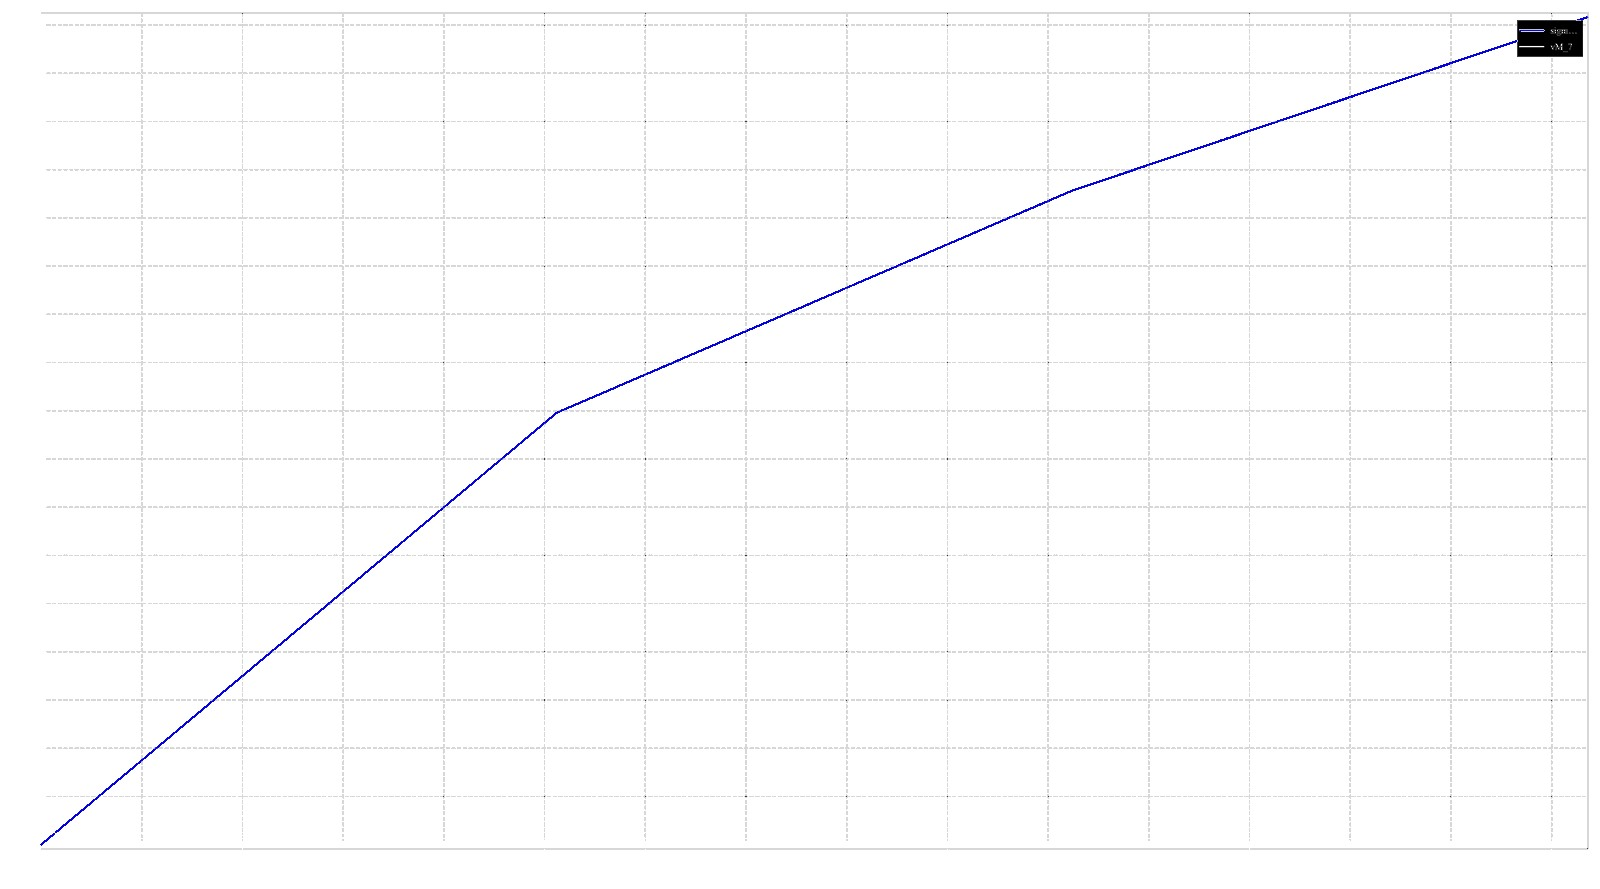
\includegraphics[width=0.85\textwidth]{images/bus7SVCIstates_case30.jpg}
\caption{\texttt{case30}, čvor 7 (SVC Type I): stanje regulatora $\sigma$ tokom
tranzijenta, u skladu sa Milano jednačinom 19.3.}
\label{fig:case30-bus7-states}
\end{figure}

\begin{figure}[H]
\centering
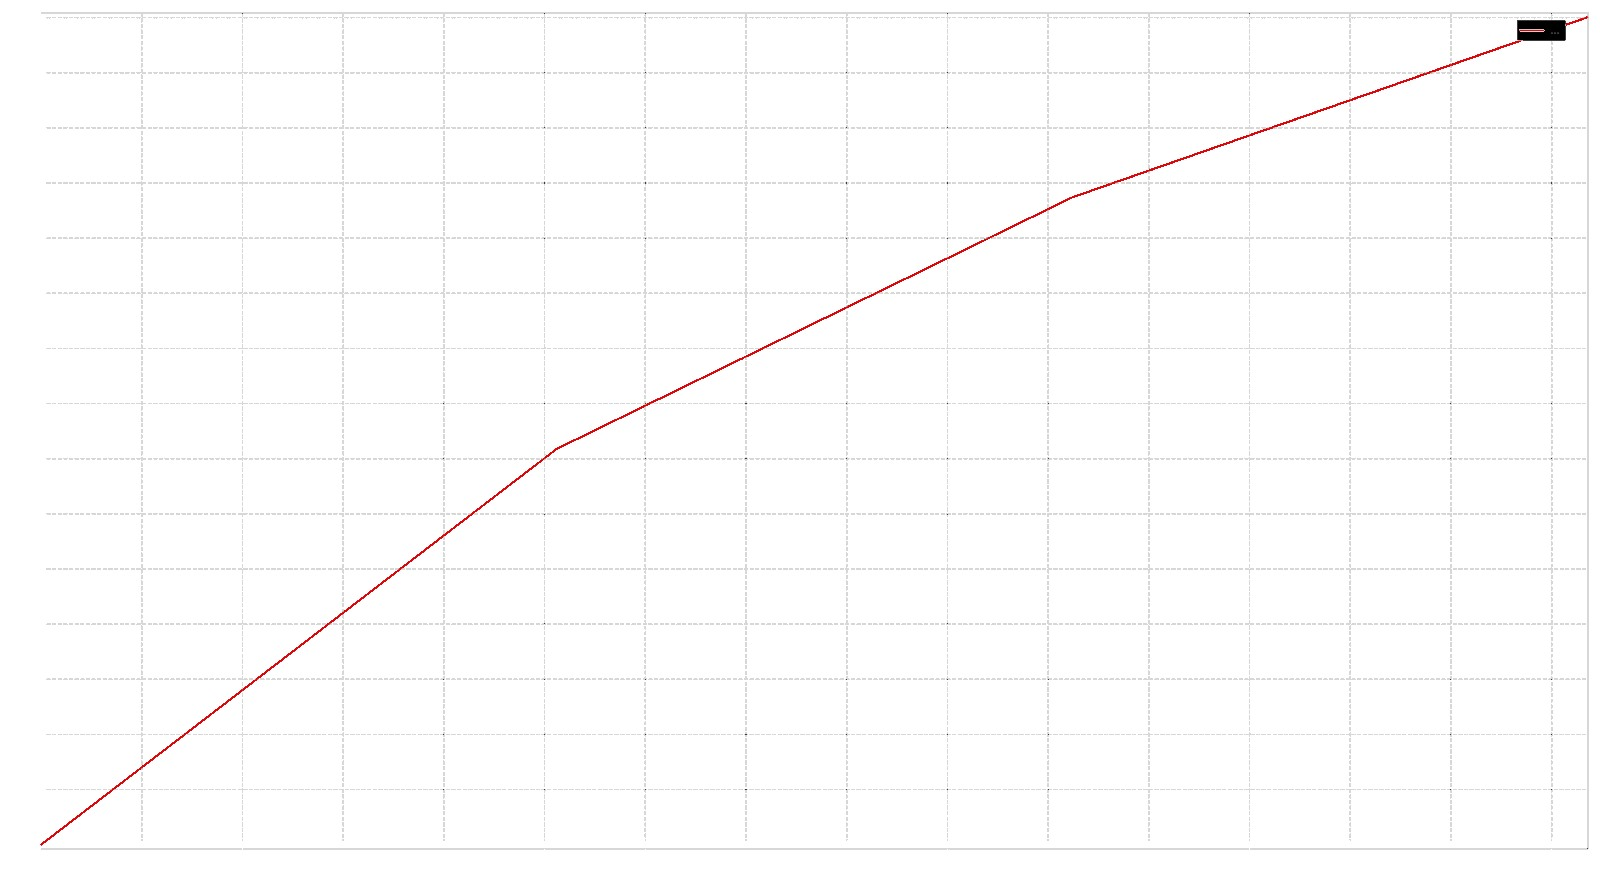
\includegraphics[width=0.85\textwidth]{images/bus7SVCQ_case30.jpg}
\caption{\texttt{case30}, čvor 7 (SVC Type I): injektirana reaktivna snaga $q$ tokom
tranzijenta.}
\label{fig:case30-bus7-q}
\end{figure}

\begin{figure}[H]
\centering
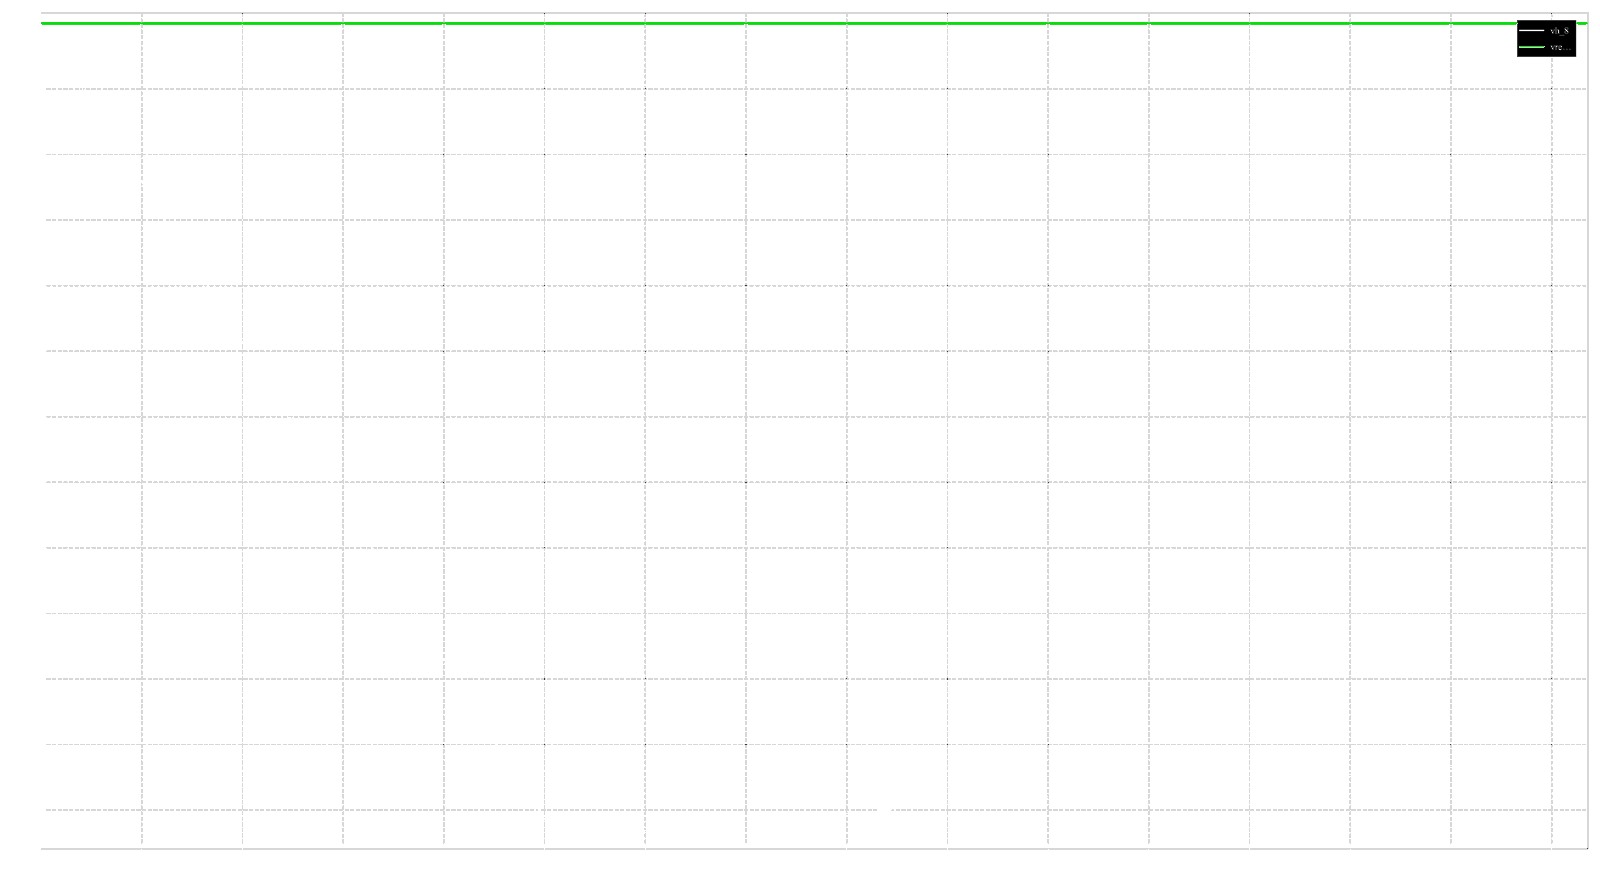
\includegraphics[width=0.85\textwidth]{images/bus8voltage_case30.jpg}
\caption{\texttt{case30}, čvor 8 (SVC Type II): napon $v_h$ naspram referentne
vrijednosti $v_{ref}$.}
\label{fig:case30-bus8-v}
\end{figure}

\begin{figure}[H]
\centering
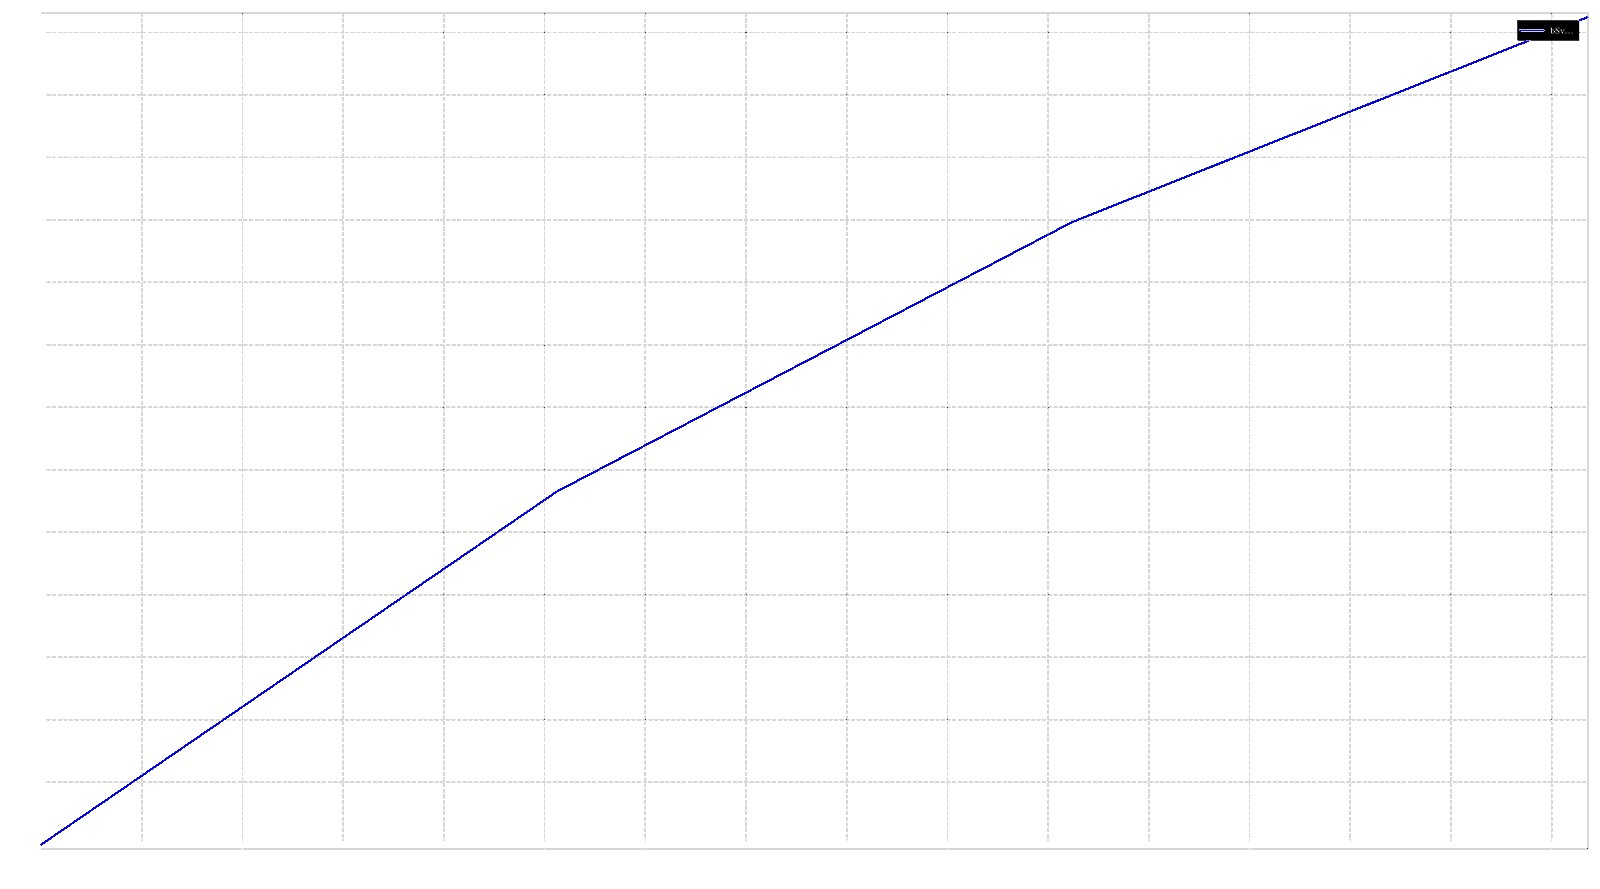
\includegraphics[width=0.85\textwidth]{images/bus8SVCIIstate_case30.jpg}
\caption{\texttt{case30}, čvor 8 (SVC Type II): stanje susceptanse $B_{SVC}$ tokom
tranzijenta (Milano eq. 19.4).}
\label{fig:case30-bus8-state}
\end{figure}

\begin{figure}[H]
\centering
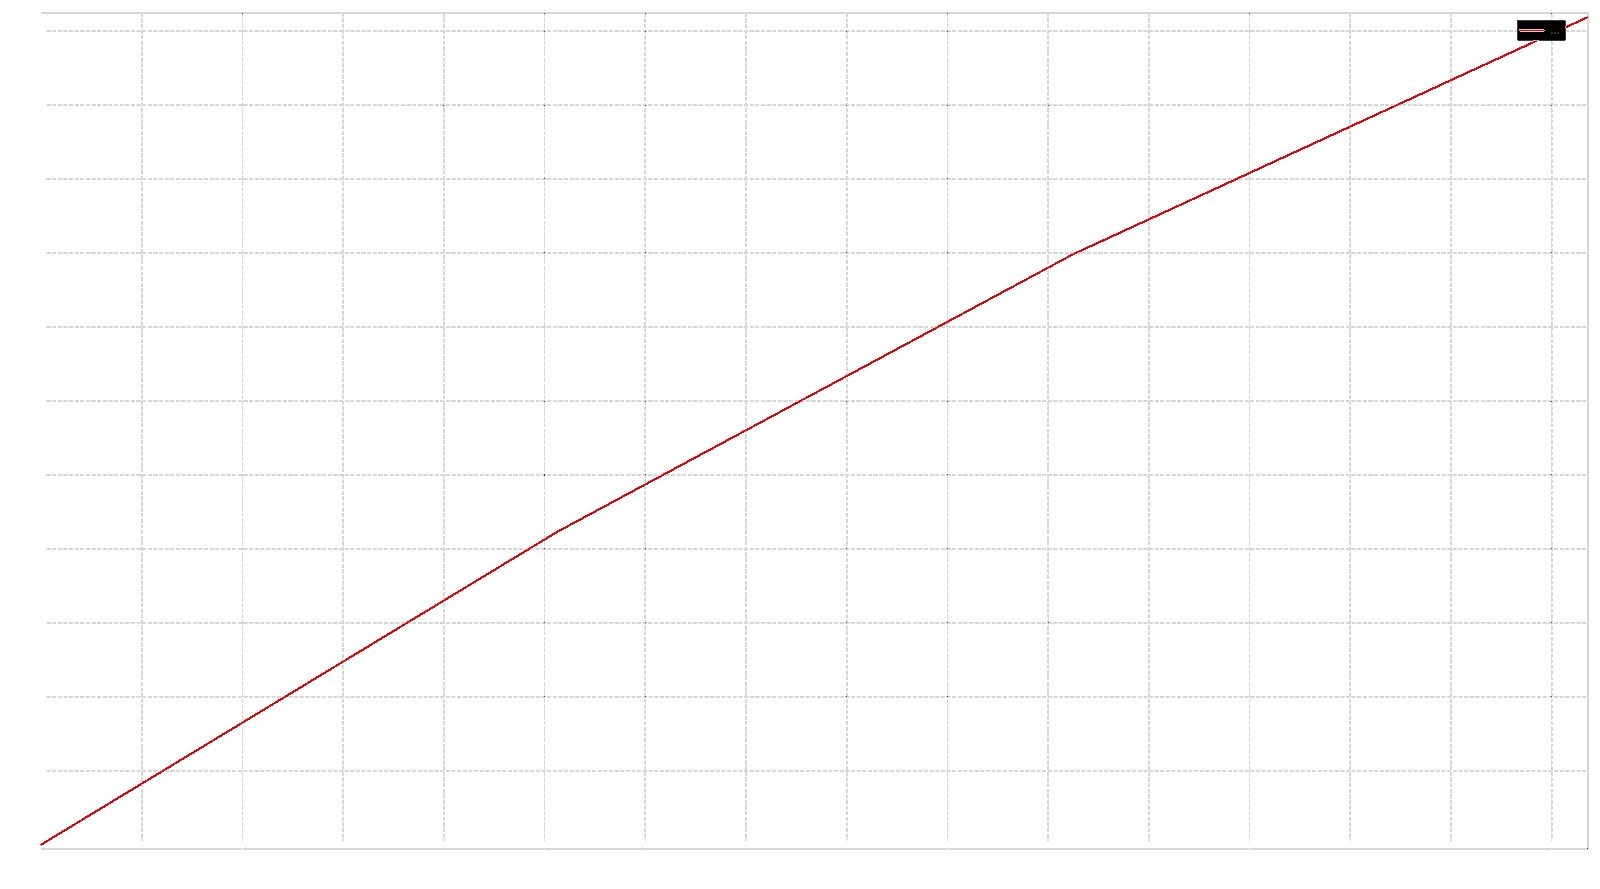
\includegraphics[width=0.85\textwidth]{images/bus8SVCQ_case30.jpg}
\caption{\texttt{case30}, čvor 8 (SVC Type II): injektirana reaktivna snaga $q$ tokom
tranzijenta.}
\label{fig:case30-bus8-q}
\end{figure}

\begin{figure}[H]
\centering
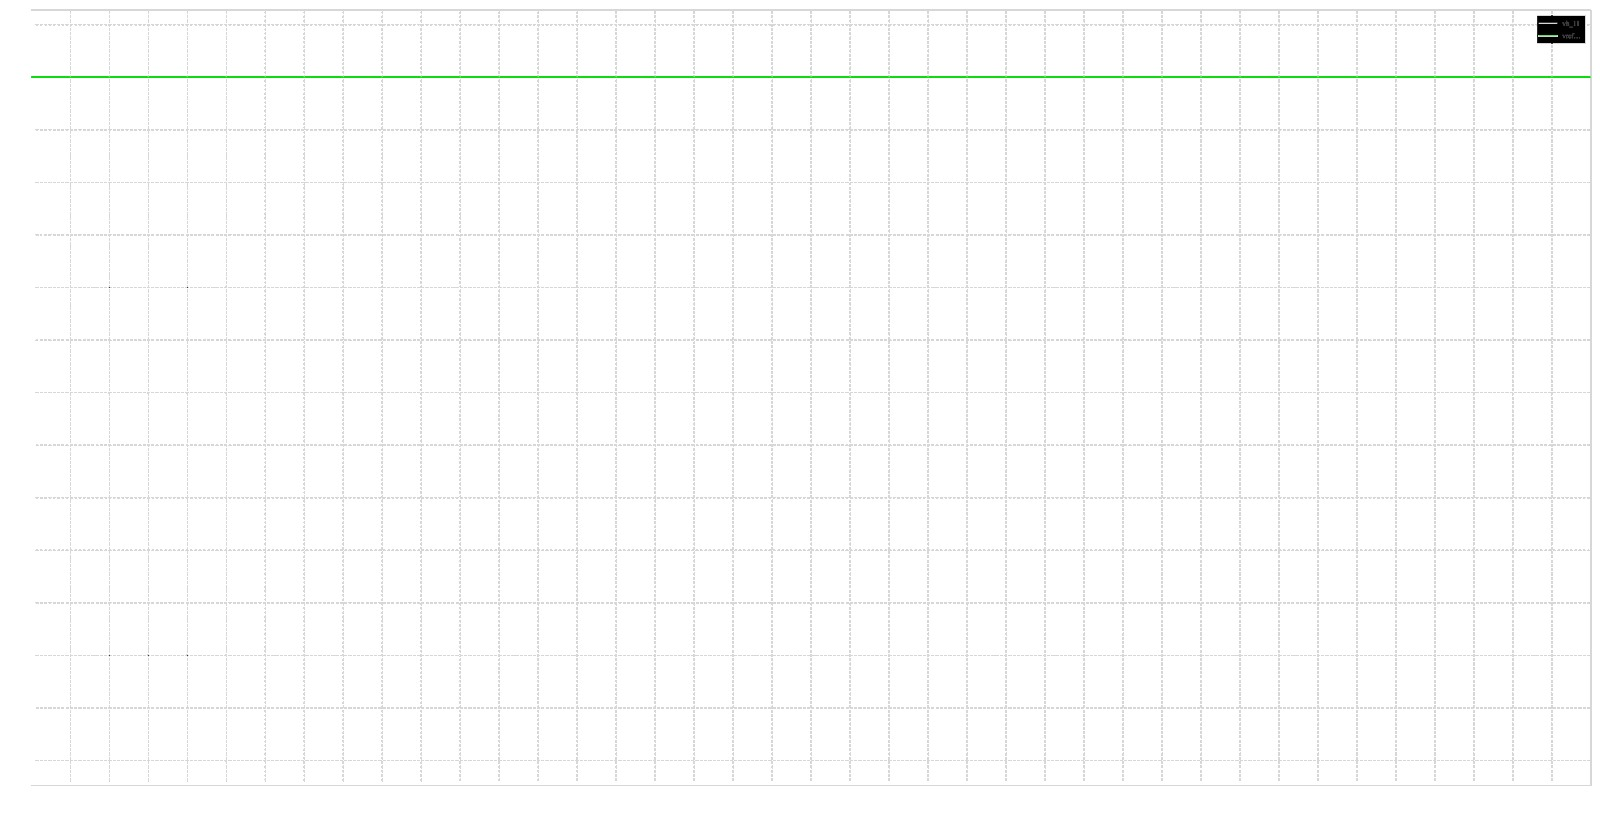
\includegraphics[width=0.85\textwidth]{images/bus11voltage_case118.jpg}
\caption{\texttt{case118}, čvor 11 (SVC Type I): napon $v_h$ naspram referentne
vrijednosti $v_{ref}$.}
\label{fig:case118-bus11-v}
\end{figure}

\begin{figure}[H]
\centering

\includegraphics[width=0.85\textwidth]{images/bus11SVCIstates_case118.jpg}
\caption{\texttt{case118}, čvor 11 (SVC Type I): stanje regulatora $\sigma$ tokom
tranzijenta.}
\label{fig:case118-bus11-states}
\end{figure}

\begin{figure}[H]
\centering

\includegraphics[width=0.85\textwidth]{images/bus11SVCIQ_case118.jpg}
\caption{\texttt{case118}, čvor 11 (SVC Type I): injektirana reaktivna snaga $q$ tokom
tranzijenta.}
\label{fig:case118-bus11-q}
\end{figure}

\begin{figure}[H]
\centering
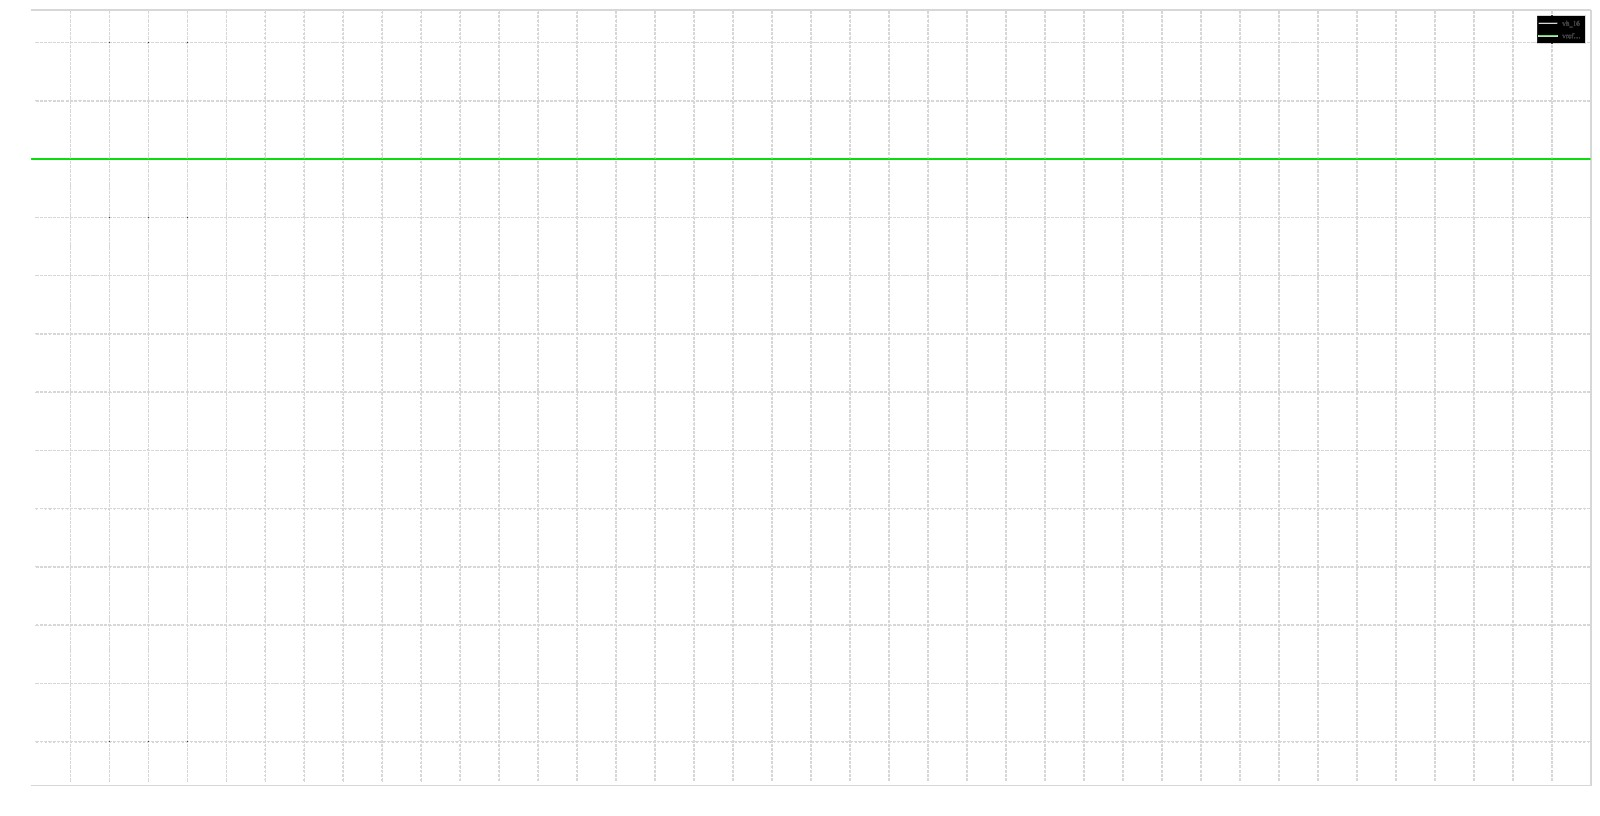
\includegraphics[width=0.85\textwidth]{images/bus16voltage_case118.jpg}
\caption{\texttt{case118}, čvor 16 (SVC Type II): napon $v_h$ naspram referentne
vrijednosti $v_{ref}$.}
\label{fig:case118-bus16-v}
\end{figure}

\begin{figure}[H]
\centering

\includegraphics[width=0.85\textwidth]{images/bus16SVCIIstate_case118.jpg}
\caption{\texttt{case118}, čvor 16 (SVC Type II): stanje susceptanse $B_{SVC}$ tokom
tranzijenta - klasičan odziv sistema prvog reda (Milano eq. 19.4), sa brzim smirivanjem
na ravnotežnu vrijednost.}
\label{fig:case118-bus16-state}
\end{figure}

\begin{figure}[H]
\centering

\includegraphics[width=0.85\textwidth]{images/bus16SVCQ_case118.jpg}
\caption{\texttt{case118}, čvor 16 (SVC Type II): injektirana reaktivna snaga $q$ tokom
tranzijenta.}
\label{fig:case118-bus16-q}
\end{figure}

Oba regulatora se ponašaju u skladu sa teorijskim očekivanjima iz Poglavlja
\ref{ch:teorija}. Kod \texttt{case118} (Slika \ref{fig:case118-bus16-state}), SVC Type II
regulator na čvoru 16 pokazuje klasičan brz odziv sistema prvog reda i smiruje se na
ravnotežnu vrijednost unutar simuliranog perioda. Kod \texttt{case30} (Slike
\ref{fig:case30-bus7-states} i \ref{fig:case30-bus8-state}), tranzijent na oba čvora je
sporiji u odnosu na zadane vremenske konstante regulatora - stanja $\sigma$ i $B_{SVC}$
još uvijek rastu na kraju 10-sekundnog perioda simulacije, što ukazuje da bi za ovaj manji
i slabije povezan test slučaj (30 čvorova, veće ekvivalentne impedanse mreže) trebalo
produžiti \texttt{endTime} u XML konfiguraciji kako bi se u potpunosti dostiglo
ravnotežno stanje.


% =============================================================================
\chapter{Zaključak}
\label{ch:zakljucak}
% =============================================================================

U ovom radu implementiran je natID/dTwin plugin koji automatski konvertuje statički
MATPOWER model mreže u dinamički DAE model sa SVC Type I i/ili SVC Type II dinamikom na
proizvoljno odabranim čvorovima, uz potpunu konfigurabilnost preko XML fajla. Cjelokupan
proračunski pipeline (parsiranje ulaznih podataka, izgradnja matrice admitansi,
generisanje diferencijalno-algebarskih jednačina) implementiran je koristeći isključivo
natID-ove \texttt{dense} i \texttt{sparse} matrice, u skladu sa zahtjevima predmeta.
Konverzija se izvršava u zasebnom thread-u, sa napretkom koji se u realnom vremenu
prikazuje u GUI-u glavnog thread-a preko \texttt{gui::thread::\allowbreak asyncExecInMainThread}
mehanizma.

Testiranje u pravom dTwin okruženju (Poglavlje \ref{ch:testiranje})
potvrdilo je da se ponašanje oba tipa SVC regulatora poklapa sa teorijskim očekivanjima iz
Milano \cite{milano2010psms}: oba regulatora uspješno vraćaju napon na zadatu referentnu
vrijednost, uz karakterističan prebačaj kod direktne regulacije susceptanse (Type II).
Konverzija najvećeg test slučaja (\texttt{case300}, 300 čvorova) traje reda veličine
nekoliko sekundi (parsiranje generisanog \texttt{.dmodl} fajla oko 65ms, inicijalizacija
oko 31ms), dok samo rješavanje tranzijentne simulacije (10s simuliranog vremena) traje
ispod jedne sekunde (oko 938ms), a ukupno vrijeme (parsiranje + init + rješavanje +
izvještavanje) iznosi oko 1.24 sekunde - i pored \texttt{report=AllDetails} logovanja svih
iteracija.


\begin{thebibliography}{9}

\bibitem{milano2010psms}
F. Milano, \emph{Power System Modelling and Scripting}, Power Systems series,
Springer-Verlag Berlin Heidelberg, 2010. (Poglavlje 19: FACTS Devices, odjeljak 19.1
Static Var Compensator).

\bibitem{acha2004facts}
E. Acha, C. R. Fuerte-Esquivel, H. Ambriz-Perez, C. Angeles-Camacho, \emph{FACTS:
Modelling and Simulation in Power Networks}, Wiley, 2004.

\bibitem{natid}
I. Džafić, \emph{natID - native Interface Design}, \url{https://github.com/idzafic}.

\bibitem{matpower}
R. D. Zimmerman, C. E. Murillo-Sanchez, \emph{MATPOWER}, \url{https://matpower.org}.

\end{thebibliography}

\end{document}
